\documentclass{article}
\usepackage{graphicx}
\graphicspath{ {images/} }

% Latex commands
    \newcommand{\mat}[2][ccccccccccccccccccccccccccccccccccccccccccccc]{\left[
        \arraycolsep=1.2pt\def\arraystretch{1.5}
        \begin{array}{#1} #2 \\ 
        \end{array} 
        \right]}

        %% Miscelaneous commands
        
        %% Tool tracking positions
        \newcommand{\xbT}{\vec{x}{^b_T}} % tool tip in body coords
        \newcommand{\xwT}{\vec{x}{^w_T}} % tool tip in world coords
        \newcommand{\xcT}{\vec{x}{^c_T}} % tool tip in camera coords
        \newcommand{\xwE}{\vec{x}{^w_E}} % eraser in world coords
        \newcommand{\xcE}{\vec{x}{^c_E}} % eraser in camera coords

        %% Tool tracking orientations
        \newcommand{\q}[3]{{^#1}\vec{q}{^#2_#3}} % eraser in world coords

        %% Rotation and Translation vectors
        \newcommand{\R}[2]{{^#1}{\bf{R}}{^#2}}
        \newcommand{\T}[2]{{^#1}{\vec{t}}{^#2}}

\begin{document}

\begin{flushleft}

%%%%%%%%%%%%%%%%%%%%%%%%%%%%%%%%%%%%%%%%%%%%%%%%%%%%%%%%%%%%%%%%%%%%%%%%%%%%%%%
%%%%% Tool Model
%%%%%%%%%%%%%%%%%%%%%%%%%%%%%%%%%%%%%%%%%%%%%%%%%%%%%%%%%%%%%%%%%%%%%%%%%%%%%%%

\medskip

The position of the tip of the interaction tool is $ \xwT $. This position is specified in world coordinates; the superscript $w$ indicates that the coordinates of this position are specified relative to the origin of world space, $\bf{O_w}$. The origin of the world coordinate system is the head of the user who is wearing a virtual reality display. This is not exactly the position of the camera, though the two coordinate systems correspond. The origin of the camera coordinate system, $\bf{O_c}$, is offset from the world coordinate system by the rotation and translation of the user's head. The rotation and translation of the user's head will be minimal while the user is seated. 

\medskip

Let $\R{c}{w}$ and $\T{c}{w}$ be the rotation and translation matrices, respectively, that specify the transformation from the world coordinate system to the camera coordinate system. Then the position of the interaction tool in camera coordinates, $ \xcT $,  is given by the following relation: 

\[ \xcT = \R{c}{w} \xwT + \T{c}{w} \]

The position of the tool relative to the camera, $ \xcT $, is not observed directly. However, this position is inferred from the position of the back of the tool, $ \xcE $, and the orientation of the tool, $ \q{c}{b}{T} $. Call the back of the tool the eraser. The position of the eraser is found through computer vision; the orientation of the tool is found through filtering of data from an inertial measurement unit on the tool. The position of the tool is found through the following relation: 

\[ \xcT = \xcE + \mat{ \bf{I_3} & \vec{0} }\q{c}{w}{T} ( \q{w}{b}{T} \mat{ 0 \\ \ell \xbT} \q{w}{b}{T}^{*} ) \q{c}{w}{T}^{*} \]


\medskip
%%%%%%%%%%%%%%%%%%%%%%%%%%%%%%%%%%%%%%%%%%%%%%%%%%%%%%%%%%%%%%%%%%%%%%%%%%%%%%%
%%%%% Camera Model
%%%%%%%%%%%%%%%%%%%%%%%%%%%%%%%%%%%%%%%%%%%%%%%%%%%%%%%%%%%%%%%%%%%%%%%%%%%%%%%
\medskip





\medskip
%%%%%%%%%%%%%%%%%%%%%%%%%%%%%%%%%%%%%%%%%%%%%%%%%%%%%%%%%%%%%%%%%%%%%%%%%%%%%%%
%%%%% Camera Model
%%%%%%%%%%%%%%%%%%%%%%%%%%%%%%%%%%%%%%%%%%%%%%%%%%%%%%%%%%%%%%%%%%%%%%%%%%%%%%%
\medskip
The following is a model of a single frame from the camera. In this frame,
the red circular object represents the back of the interaction tool. The back
of the interaction tool is called the target. The width of the target along
the $x$ dimension of the image is $d_{ux}$ and the width along the $y$ 
dimension is $d_{uy}$. The midpoint of the target is 
$\bf{\vec{x_U}} = \mat{ x_y & y_u }^{T}$.

\medskip

\begin{center}
    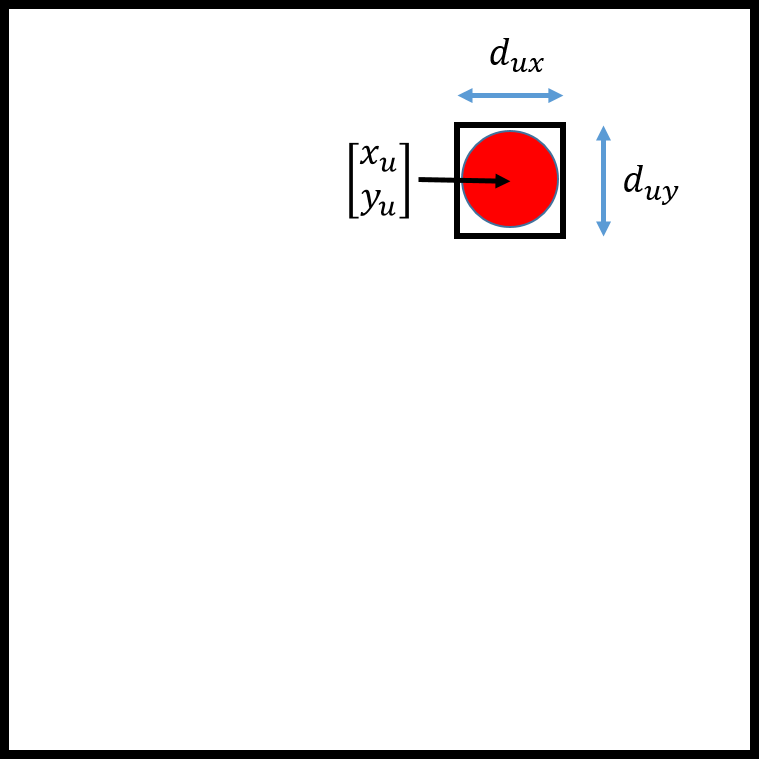
\includegraphics[scale=0.4]{cameraMeasurement}
\end{center}

\medskip

These measurements are related to the hidden state $\bf{\vec{x_C}} = 
\mat{ x_C & y_C & z_C }^{T}$ in the following way: 

\[
    \bf{\vec{y}} = h(\bf{\vec{x}})
         = \mat{x_u \\ y_u \\ d_{ux} \\ d_{uy}} 
     = \mat{ \frac{f_x x_c}{z_c} \\ 
             \frac{f_y y_c}{z_c} \\ 
             \frac{d_c}{z_c \sqrt{\frac{1}{f_x^{2}} + \frac{1}{f_y^{2}}}} \\
             \frac{d_c}{z_c \sqrt{\frac{1}{f_x^{2}} + \frac{1}{f_y^{2}}}}
           }
\]

\end{flushleft}

\end{document}

% Example latex schemas
% Example for using left/right scripts \[{^g}{p}{} = ({^b}{R}{^w_l})^2+{^g}{o}{_l}\]
